\documentclass{article}
\usepackage[utf8]{inputenc}
\usepackage[margin=2cm]{geometry}
\usepackage{enumitem}
\usepackage{csquotes}

% maths packages
\usepackage{amsmath}
\usepackage{amssymb}
\usepackage{amsthm}
\usepackage{braket}

% remove space between ket and bra
\renewcommand\bra[1]{{\langle{#1}|}}
\makeatletter
\renewcommand\ket[1]{
  \@ifnextchar\bra{\k@t{#1}\!}{\k@t{#1}}
}
\renewcommand\ket[1]{
  \@ifnextchar\braket{\k@t{#1}\!}{\k@t{#1}}
}
\newcommand\k@t[1]{{|{#1}\rangle}}
\makeatother

% graphics packages
\usepackage{graphicx}
\usepackage{subcaption}
\usepackage[font={small,it}]{caption}
\usepackage{tikz}
\usetikzlibrary{positioning, circuits.logic.US}

% tikz ellipse arcs
\tikzset{
    partial ellipse/.style args={#1:#2:#3}{
        insert path={+ (#1:#3) arc (#1:#2:#3)}
    }
}

\title{Introduction to quantum information theory}
\author{Suzie Brown}
\date{\today}

% bibliography
\usepackage[round, sort&compress]{natbib}
\usepackage{har2nat} %%% Harvard reference style
\bibliographystyle{agsm}

% theorems
\newtheorem{thm}{Theorem}
\newtheorem{lemma}{Lemma}
\newtheorem{cor}{Corollary}
\theoremstyle{definition}
\newtheorem{defn}{Definition}
\newtheorem{example}{Example}

% probability symbols
\newcommand{\PR}{\mathbb{P}}
\newcommand{\E}{\mathbb{E}}
\newcommand{\V}{\operatorname{Var}}
\newcommand{\iidsim}{\overset{iid}{\sim}}
\newcommand{\eqdist}{\overset{d}{=}}

% distributions
\newcommand{\Bern}{\operatorname{Bernoulli}}
\newcommand{\Geom}{\operatorname{Geom}}

% project-specific commands
\newcommand{\A}{\mathcal{A}}
\newcommand{\AND}{{\footnotesize AND }}
\newcommand{\NAND}{{\footnotesize NAND }}
\newcommand{\OR}{{\footnotesize OR }}
\newcommand{\NOR}{{\footnotesize NOR }}
\newcommand{\NOT}{{\footnotesize NOT }}

\begin{document}
\maketitle

\section{Quantum information}\label{sec:quantum_info}
This section is based on the course by Noah Linden (University of Bristol) and discussion with Thomas Hebdige and David Jennings (Imperial College London). For a comprehensive introduction see for example \citet{nielsen2002} or \citet{wilde2013}.

The basis of quantum mechanics is simply linear algebra in a Hilbert space. The definitions in Sections \ref{sec:hilbert_defn} to \ref{sec:linear_ops} are exactly what you would find in a linear algebra course, except for the notation. 
The famously strange quantum behaviour arises from the ``rules of quantum mechanics'' (Section \ref{sec:rules_of_qm}) pertaining to measurements. The majority of phenomena besides are described perfectly naturally by linear algebra, and are only counter-intuitive when one departs from the safety of mathematical abstraction and attempts to interpret quantum behaviour within the framework of the natural world, as perceived on a human scale. 
It is not surprising that such attempts should lead to confusion, since quantum mechanics is based on complex numbers and so diverges from human reality even at its very fundamentals.

\subsection{Dirac notation}
Dirac notation is a convenient way of denoting vectors such that it is easy to visually identify inner and outer products, and thus quickly recognise scalars, vectors and matrices:

\begin{itemize}
\item $\ket{v}$ denotes a column vector
\item $\bra{v}$ denotes a row vector
\item $\braket{u|v}$ denotes an inner product (resulting in a scalar)
\item $\ket{u}\bra{v}$ denotes an outer product (resulting in a matrix)
\end{itemize}
Additionally, $\overline{\alpha}$ denotes the complex conjugate of a scalar $\alpha$, and $U^\dag$ denotes the adjoint (conjugate transpose) of an operator $U$.

\subsection{Hilbert space}\label{sec:hilbert_defn}
A \emph{Hilbert space} is a vector space with an inner product $\braket{\cdot|\cdot}$ satisfying the following:
\begin{itemize}
\item $\bra{u} \left(\alpha\ket{v} + \beta\ket{w}\right) = \alpha\braket{u|v} + \beta\braket{u|w}$
\item $\braket{u|v} = \overline{\braket{v|u}}$
\item $\braket{v|v} \geq 0$ with equality if and only if $\ket{v}$ is the zero vector.
\end{itemize}

\subsection{Orthonormal bases}\label{sec:onb}
An \emph{orthonormal basis} of a Hilbert space $\mathcal{H}$ is a set of vectors $\{v_1,\dots,v_n\}$ in $\mathcal{H}$ such that:
\begin{itemize}
\item $\operatorname{span} \{v_1,\dots,v_n\} = \mathcal{H}$
\item $\braket{v_i|v_j} = \delta_{ij}$
\end{itemize}
We now restrict to the Hilbert space $\mathbb{C}^2$, which is the state space of a single quantum bit (qubit), and is sufficient to describe the basics of quantum information. The \emph{computational basis} $\{\ket{0}, \ket{1}\} = \{(1,0)^T,(0,1)^T\}$ is taken as the canonical basis for $\mathbb{C}^2$ and is henceforth used wherever not specified otherwise. Since it is an orthonormal basis, every vector $\ket{v}$ in $\mathbb{C}^2$ has a unique representation
\begin{equation*}
\ket{v} = \alpha \ket{0} + \beta \ket{1} \equiv (\alpha,\beta)^T
\end{equation*}
for some $\alpha, \beta \in \mathbb{C}$. For reasons which will probably not become apparent in this treatment, we restrict ourselves to \emph{normalised} vectors, requiring also $|\alpha|^2 + |\beta|^2 = 1$.
We will also consider two vectors equivalent if they differ only by an overall phase, i.e.\ $\ket{u} \equiv \ket{v}$ if $\ket{u} = e^{i\theta}\ket{v}$ for some $\theta$, since it is impossible to distinguish between two such vectors with any measurement.

To ensure coherency with the properties of the inner product, we have that
\begin{equation*}
\bra{v} = \overline{\alpha} \bra{0} + \overline{\beta} \bra{1}.
\end{equation*}
The inner product of $\ket{v} = \alpha \ket{0} + \beta \ket{1}$ with $\ket{u} = \gamma \ket{0} + \delta \ket{1}$ is therefore computed as
\begin{align*}
\braket{v|u} &= (\overline{\alpha}\bra{0} + \overline{\beta}\bra{1}) (\gamma\ket{0} + \delta\ket{1})\\
&= \overline{\alpha}\gamma\braket{0|0} + \overline{\alpha}\delta\braket{0|1} + \overline{\beta}\gamma\braket{1|0} + \overline{\beta}\delta\braket{1|1} \\
&= \overline{\alpha}\gamma + \overline{\beta}\delta.
\end{align*}
One alternative choice of orthonormal basis which is worth mentioning is given by $\{\ket{+},\ket{-}\}$, consisting of the states
\begin{align*}
&\ket{+} := \frac{1}{\sqrt{2}}(\ket{0} + \ket{1}) \\
&\ket{-} := \frac{1}{\sqrt{2}}(\ket{0} - \ket{1}).
\end{align*}

\subsection{Linear operators}\label{sec:linear_ops}
A linear operator is an operator with the property
\begin{equation*}
A \left(\alpha\ket{u} + \beta\ket{v}\right) = \alpha A\ket{u} + \beta A\ket{v}.
\end{equation*}
It is therefore fully defined by its action on an orthonormal basis. For instance, the quantum \NOT operator (usually denoted $X$) is defined by
\begin{align*}
& X\ket{0} = \ket{1} \\
& X\ket{1} = \ket{0}
\end{align*}
Equivalently, $X$ can be expressed as a matrix with respect to the computational basis:
\begin{equation*}
X = \begin{pmatrix}
0 & 1 \\ 1 & 0
\end{pmatrix}
\end{equation*}
In Dirac notation, operators are written in terms of outer products of basis states:
\begin{equation*}
X = \ket{0}\bra{1} + \ket{1}\bra{0}
\end{equation*}
This is equivalent to the matrix form:
\begin{equation*}
X = \begin{pmatrix}1\\0 \end{pmatrix} \begin{pmatrix} 0&1 \end{pmatrix}
+ \begin{pmatrix}0\\1 \end{pmatrix} \begin{pmatrix} 1&0 \end{pmatrix}
= \begin{pmatrix} 0 & 1 \\ 0 & 0 \end{pmatrix} +  \begin{pmatrix} 0 & 0 \\ 1 & 0 \end{pmatrix}
= \begin{pmatrix} 0 & 1 \\ 1 & 0 \end{pmatrix}.
\end{equation*}
Then the action of $X$ on a general state $\ket{v} = \alpha \ket{0} + \beta \ket{1}$ can be calculated:
\begin{align*}
X\ket{v} &= (\ket{0}\bra{1} + \ket{1}\bra{0})(\alpha \ket{0} + \beta \ket{1})\\
&= \alpha \ket{0}\braket{1|0} + \alpha \ket{1}\braket{0|0} + \beta \ket{0}\braket{1|1} +
\beta \ket{1}\braket{0|1}\\
&= \alpha \ket{1} + \beta \ket{0}.
\end{align*}

\begin{defn}
Let $U$ be a linear operator.
\begin{itemize}
\item $U$ is said to be \emph{self-adjoint} (or \emph{hermitian}) if $U^\dag = U$.
\item $U$ is said to be \emph{unitary} if $UU^\dag = U^\dag U = I$.
\end{itemize}
\end{defn}

For example, the operator $X$ is both self-adjoint and unitary. Crucially, unitary operators preserve normalisation, so they map states to states. It is also obvious that unitary transformations are always reversible (i.e.\ the inverse operator exists).

\subsection{Rules of Quantum Mechanics}\label{sec:rules_of_qm}
\begin{enumerate}
\item \emph{States} of a quantum mechanical system correspond to normalised vectors in Hilbert space, up to an overall phase.
\item \emph{Evolutions} of the system correspond to unitary operators.
\item \emph{Measurements} on quantum states correspond to self-adjoint operators --- see below.
\end{enumerate}

\subsubsection{Spectral theorem and measurement}\label{sec:quantum_mmt}
The outcome of a measurement depends on the current state of the system and the type of measurement performed (i.e.\ which self-adjoint oeprator is applied).
The spectral theorem states that every self-adjoint operator $A$ can be represented by its spectral decomposition
\begin{equation}\label{eq:operator_diag}
A = \sum_{i} \lambda_i P_i
\end{equation}
where $\{\lambda_1,\dots, \lambda_k\}$ is the set of \emph{distinct} eigenvalues of $A$, and $P_i$ is the \emph{projection} operator onto the eigenspace corresponding to eigenvalue $\lambda_i$.

When we measure a state $\ket{x}$ using operator $A$, the measurement outcome we observe is one of the eigenvalues of $A$. In particular, we observe $\lambda_i$ with probability $\bra{x} P_i \ket{x}$.
Making a measurement causes the system to collapse onto the eigenspace corresponding to the observed eigenvalue; that is, the state after measurement is proportional to $P_i \ket{x}$.\\

\begin{example}\label{ex:quantum_mmt}
To give a concrete example, let us consider again the operator $X$. This operator has eigenvalues $\pm 1$ corresponding to eigenvectors (or \emph{eigenstates} in quantum mechanics) $\ket{+}$ and $\ket{-}$ respectively.
Therefore $X$ admits the diagonal representation
\begin{equation*}
X= \ket{+}\bra{+} - \ket{-}\bra{-}
\end{equation*}
which is of the form \eqref{eq:operator_diag}.
Now suppose we make a measurement on the state $\ket{v} = \ket{0}$, using $X$.
The outcome of the measurement will be an eigenvalue of $X$: either $+1$ or $-1$. We observe the outcome $+1$ with probability
\begin{equation*}
\bra{v} P_{+1} \ket{v} = \braket{0|+}\braket{+|0} = 1/2
\end{equation*}
in which case the state after measurement is
\begin{equation*}
P_{+1} \ket{v} = \ket{+} \braket{+|0} \propto \ket{+}.
\end{equation*}
Similarly, with probability 1/2 we observe the outcome $-1$ and the state after measurement is $\ket{-}$.
\end{example}

In this example, the two outcomes are equally likely because the state $\ket{0}$ is `equidistant' from the two eigenstates of $X$. In general, outcomes that leave the state after measurement closer to the original state are more likely. This notion is formalised in Section \ref{sec:bloch_sphere}.

A particularly important type of measurement is measurement in the computational basis. In this case the self-adjoint operator used is $0\cdot \ket{0}\bra{0} +1\cdot \ket{1}\bra{1} = \ket{1}\bra{1}$.
Measuring a state $\ket{v}=\alpha\ket{0} + \beta\ket{1}$ in the computational basis returns 0 with probability $|\alpha|^2$ or 1 with probability $|\beta|^2$. This is useful in quantum computing algorithms because it deterministically converts the basis states $\ket{0}$ and $\ket{1}$ to their classical equivalents 0 and 1, ready for classical output.

\begin{figure}
\centering
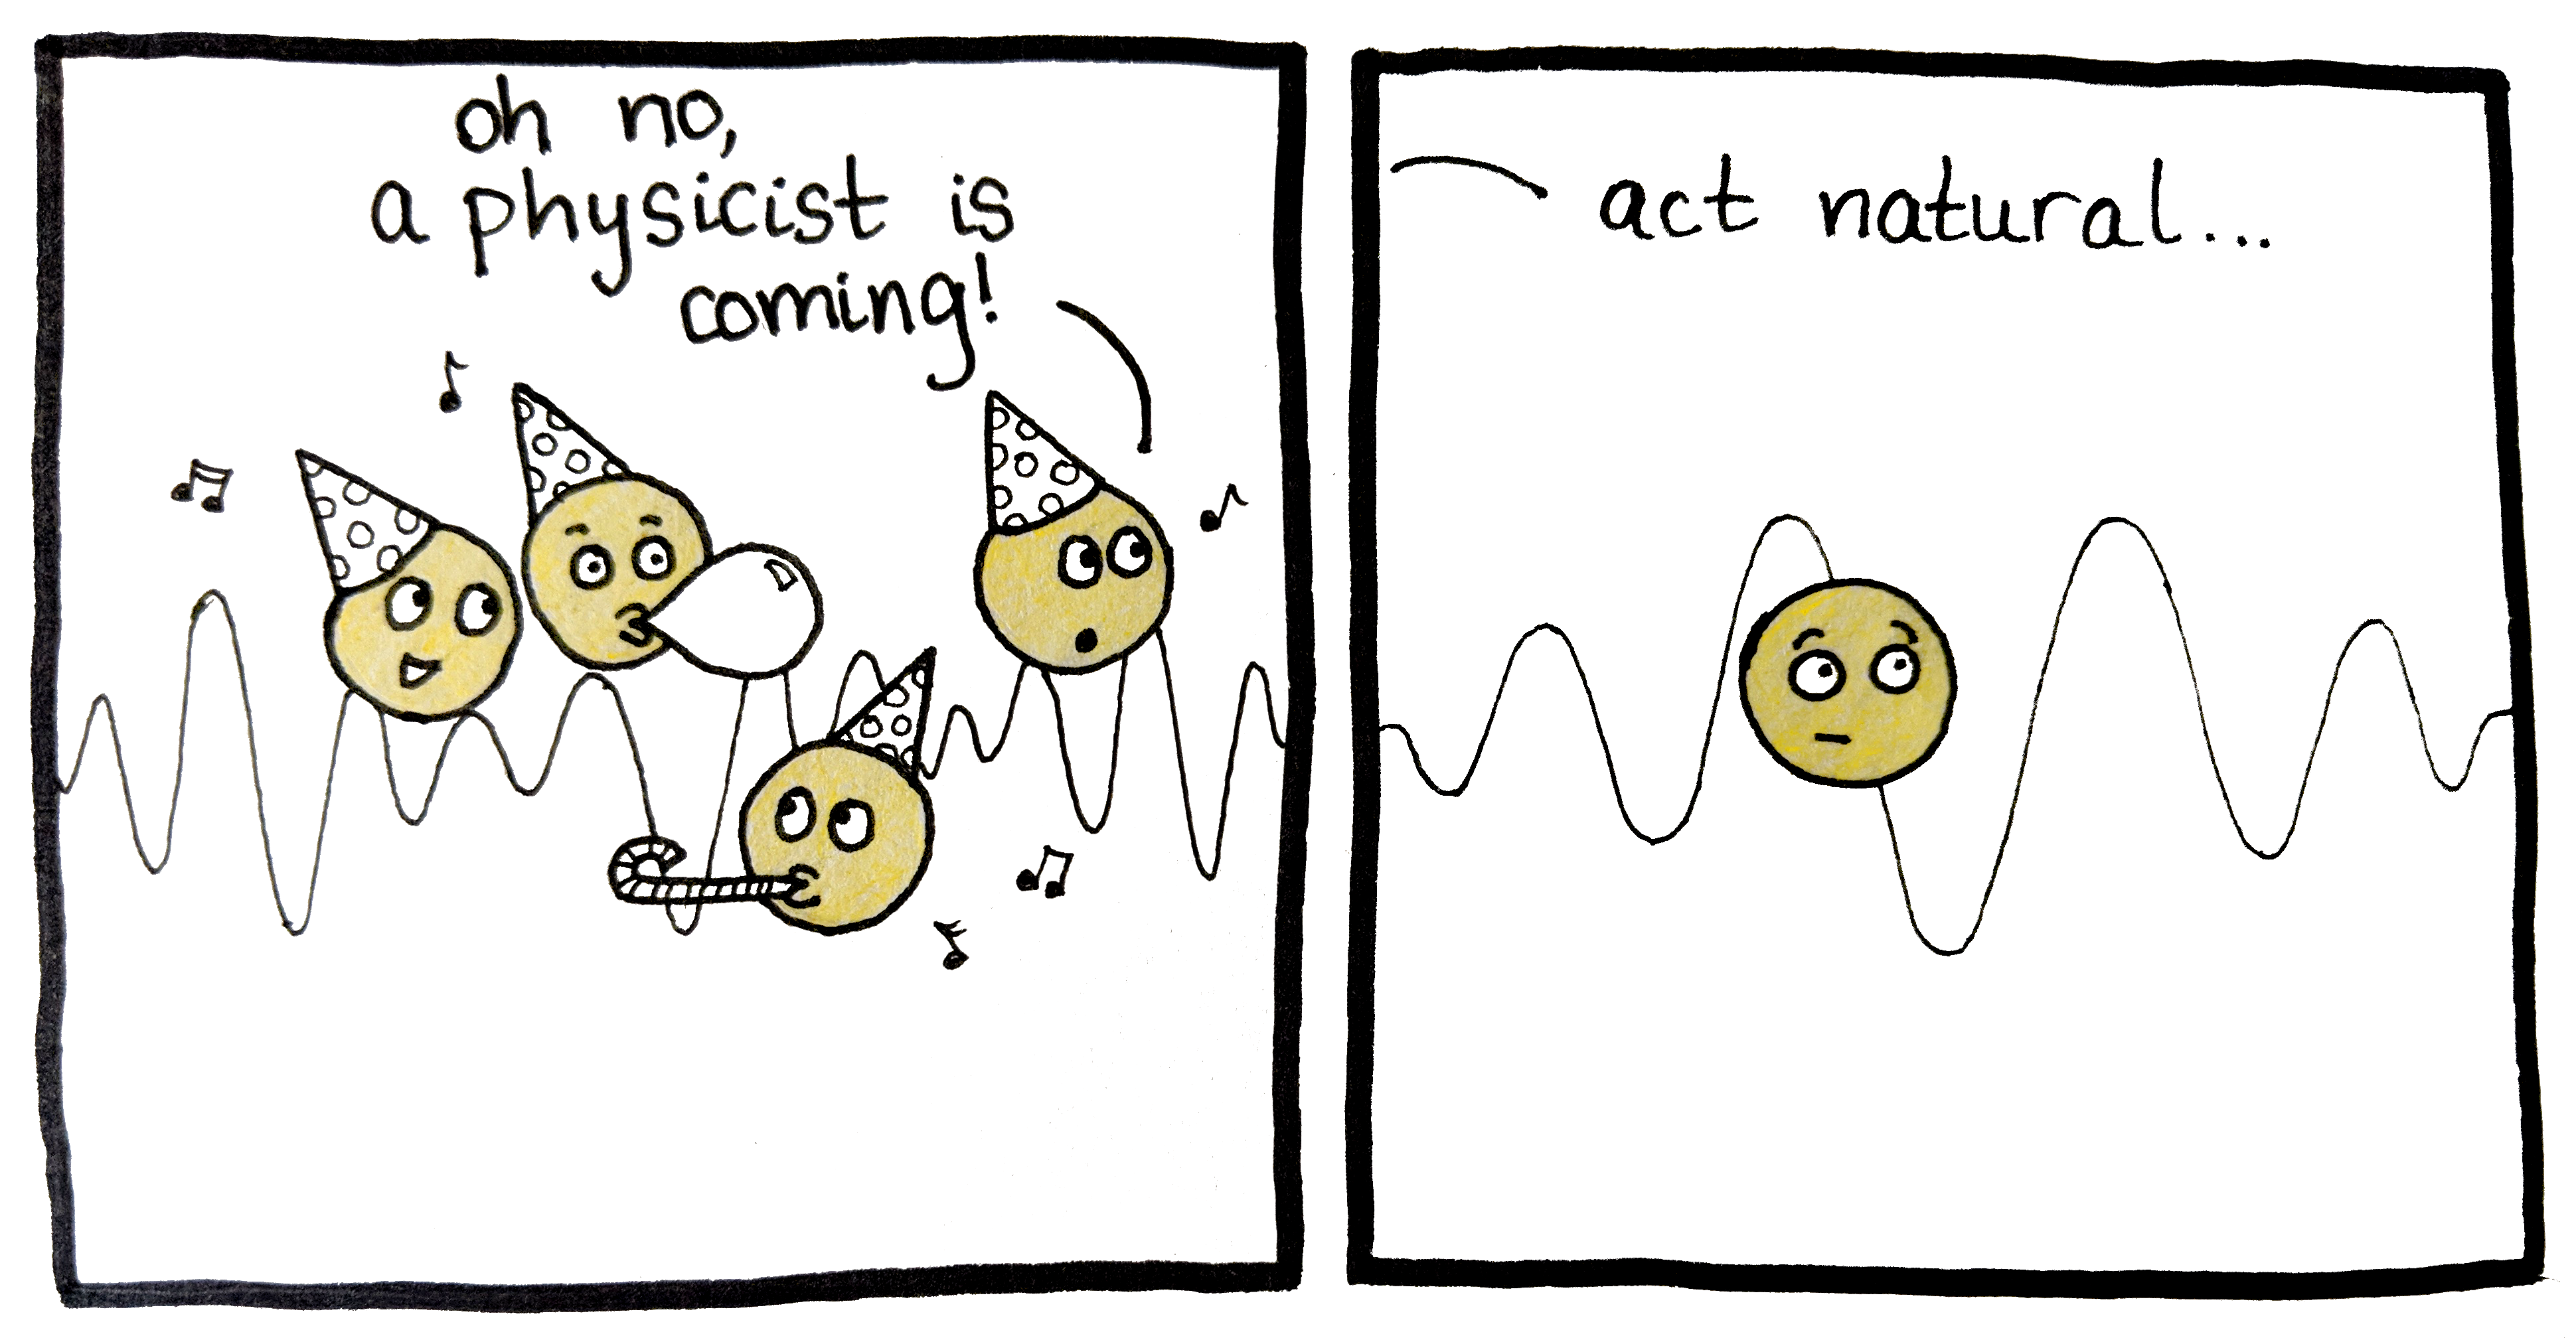
\includegraphics[width=0.8\textwidth]{qit_comic.png}
\caption{When a quantum system is in a superposition of states, making a measurement causes the system to collapse into the eigenstate corresponding to the observed eigenvalue.}
\label{fig:quantum_mmt_comic}
\end{figure}

\subsection{Quantum randomness}
It is worth remarking at this point on the difference between quantum and classical randomness.
As statisticians we are used to dealing with randomness, but we accept that randomness is simply part of a model, and is not purported to exist in nature. We artificially introduce random variables into our models to account for a lack of information, either about the state of the system or about the (presumably deterministic) processes that govern certain phenomena.

On the contrary, our uncertainty about the outcome of a measurement on a quantum system is of a different kind. This uncertainty is not a symptom of our lack of knowledge: even when we know exactly the state of the system, as in Example \ref{ex:quantum_mmt}, we are still unable to predict with certainty the outcome of a measurement on the system. The randomness here is intrinsic; the natural processes governing quantum measurement are truly stochastic.

\subsection{Pure and mixed states}
So far we have only encountered \emph{pure states}, like $\ket{0}$ or $\ket{+}$. But we can also consider probabilistic mixtures of pure states, known as \emph{mixed states}, like
\begin{equation*}
\ket{v} = \sum_{i} p_i \ket{v_i}
\end{equation*}
where $\{p_i\}$ is a probability distribution and the $\ket{v_i}$ are pure states.
You can think of this as a `source' which emits a state $\ket{v_i}$ with probability $p_i$.
A classical analogue is a bit which takes the value 1 with probability $p$ or 0 with probability $1-p$ (a $p$-coin). In this case, we can say that the expected value of the bit is $p$.

There is no full ordering on the set of quantum states, so it is not possible to define the expected value of a mixed state. However, we can calculate the expected value of a measurement on a mixed state, using the state's \emph{density operator}.

\subsubsection{Density operators}
The density operator of a mixed state $\ket{v} = \sum_{i} p_i \ket{v_i}$ is given by
\begin{equation*}
\rho = \sum_{i} p_i \ket{v_i}\bra{v_i}.
\end{equation*}
Suppose we measure this mixed state using the self-adjoint operator $A= \sum_k \lambda_k P_k$, where $\{\lambda_k\}$ are the distinct eigenvalues of $A$ and $P_k$ the projections onto the corresponding eigenspaces. Recall (from Section \ref{sec:quantum_mmt}) that the outcome of the measurement will be an eigenvalue of $A$. Applying the law of total probability, the probability of observing a particular outcome $\lambda_j$ is
\begin{equation*}
\PR(\text{observe }\lambda_j) = \sum_i p_i \bra{v_i} P_j \ket{v_i} = tr(\rho P_j)
\end{equation*}
where $tr(\cdot)$ denotes the trace of an operator.
Note that $tr(\rho)=1$ because the states are normalised and $\{p_i\}$ is a probability distribution.
The state $\rho = I/2$ is called the \emph{maximally mixed} state; it expresses complete ignorance, like a classical (1/2)-coin.

Different mixtures of states may have the same density operator, but in this case is is impossible to distinguish between them by any measurement. 
\begin{example}
For example, a source $\ket{v}$ which emits $\ket{0}$ or $\ket{1}$ each with probability 1/2 has the same density operator $\rho = I/2$ as a source $\ket{u}$ which emits $\ket{+}$ or $\ket{-}$ each with probability 1/2.
Suppose we measured both of these mixed states in the computational basis. The probability of observing the outcome 0 from $\ket{u}$ is
\begin{equation}
\bra{u}P_0\ket{u} = \frac{1}{2}\braket{0|0}\braket{0|0} + \frac{1}{2}\braket{1|0}\braket{0|1}
= 1/2
\end{equation}
while the probability of observing 0 from $\ket{v}$ is
\begin{equation}
\bra{v}P_0\ket{v} = \frac{1}{2}\braket{+|0}\braket{0|+} + \frac{1}{2}\braket{-|0}\braket{0|-}
= \frac{1}{2}\cdot\frac{1}{2} + \frac{1}{2}\cdot\frac{1}{2}  = 1/2.
\end{equation}
Therefore measurement in the computational basis can provide no information to distinguish between $\ket{u}$ and $\ket{v}$. And indeed nor can any other measurement --- proved easily by exchanging the projection operator $\ket{0}\bra{0}$ for general $P$ in the above --- so the two sources are indistinguishable.
\end{example}

\subsection{The Bloch sphere}\label{sec:bloch_sphere}
Density operators have a neat geometrical representation as points in a unit sphere (Figure \ref{fig:qubit_state_space}). This is called the \emph{Bloch sphere}, and can be thought of as the state space of a qubit.

An arbitrary pure state can be written in the form
\begin{equation*}
\ket{v} = e^{i\psi} \left[ \cos \left(\frac{\theta}{2}\right) \ket{0} + e^{i\phi} \sin \left(\frac{\theta}{2}\right) \ket{1} \right].
\end{equation*}
Since the overall phase $e^{i\psi}$ can be ignored, the state is parametrised by two angles $\theta$ and $\phi$. Taking these as spherical coordinates with unit radius, we can think of each pure state as a point on the unit sphere (or equivalently, a unit vector). Orthogonal states lie at opposite points on the Bloch sphere.

Mixed states can also be represented in the Bloch sphere. The Bloch vector for a mixed state is found by taking the weighted average of the Bloch vectors of its component pure states. Due to the triangle inequality, mixed states therefore lie strictly inside the unit sphere.
This illustrates that several different mixtures of states can have the same density operator. Quantum states are distinguishable if and only if they correspond to different points in the Bloch sphere.

There is an analogy here with classical information. The state space of a classical bit is the unit interval: its value could be 0 or 1, or we could take a probabilistic mixture of the two. The `pure' states then are 0 and 1, which lie on the `surface' of the interval, while `mixed' states lie strictly inside the interval (Figure \ref{fig:cbit_state_space}). 

Finally, unitary operators correspond to rotations of the Bloch sphere. This illustrates that unitary transformations are reversible.

\begin{figure}
\centering
\begin{subfigure}{0.25\linewidth}
\centering
\begin{tikzpicture}
\draw (0,4) -- (0,-4);
\filldraw (0,4) circle (2pt) node[anchor=south] {0};
\filldraw (0,-4) circle (2pt) node[anchor=north] {1};
\end{tikzpicture}
\caption{Classical bit}
\label{fig:cbit_state_space}
\end{subfigure}%
\begin{subfigure}{0.75\linewidth}
\centering
\begin{tikzpicture}
\draw (0,0) circle (4cm);
\draw (0,4) -- (0,-4);
\draw[gray] (-4,0) -- (4,0);
\draw[gray] (0,0) ellipse (4cm and 1.5cm);
\filldraw (0,4) circle (2pt) node[anchor=south] {$\ket{0}\bra{0}$};
\filldraw (0,-4) circle (2pt) node[anchor=north] {$\ket{1}\bra{1}$};
\filldraw (-4,0) circle (2pt) node[anchor=east] {$\ket{+}\bra{+}$};
\filldraw (4,0) circle (2pt) node[anchor=west] {$\ket{-}\bra{-}$};
%\filldraw (0,0) circle (2pt) node [anchor=west] {$I/2$};
\draw[ultra thick, ->] (0,0) -- (2,2);
\draw[dotted] (0,0) -- (2,-0.5);
\draw[dotted] (2,-0.5) -- (2,2);
%
\draw[blue] (0,0.5) arc (90:45:0.5);
\draw[red] (0,0) [partial ellipse=180:332:0.5cm and 0.25cm];
\node[red] at (-0.4,-0.4) {$\phi$};
\node[blue] at (0.3, 0.7) {$\theta$};
\end{tikzpicture}
\caption{Qubit}
\label{fig:qubit_state_space}
\end{subfigure}

\caption{State space of classical bits versus qubits. The state space of a classical bit is the line segment $[0,1]$. The `pure' states 0 and 1 are at the endpoints, and probabilistic mixtures of the two lie inbetween. The state space of a qubit is the Bloch sphere. Pure states lie on the surface of the sphere, and mixed states lie in the interior. The centre of the sphere is the maximally mixed state $\rho=I/2$.}
\end{figure}

\subsubsection{Geometric view of measurement}
\begin{figure}
\centering
\begin{tikzpicture}
\draw (-5,0) -- (5,0);
\draw (0,-0.1) -- (0,0.1);
\draw (5,0) arc (0:180:5);
\filldraw (-5,0) circle (2pt) node[anchor=east] {$\ket{0}$};
\filldraw (5,0) circle (2pt) node[anchor=west] {$\ket{1}$};
\filldraw (-3,4) circle (2pt) node[anchor=south] {$\ket{v}$};
\draw[->, line width = 1] (-3,4) -- (-3,0);
\draw[dotted] (-3,4) -- (0,0);
\draw[red] (-0.7, 0) arc (180:126:0.7);
\node[red] at (-0.8,0.3) {$\theta$};
\draw[red, <->] (-5,-0.2) -- node[anchor=north] {$x$} (-3,-0.2);
\end{tikzpicture}
\caption{When measuring a state in the computational basis, the probability of observing a certain eigenvalue is related to the projected distance $x$ from the corresponding eigenstate.}
\label{fig:bloch_mmt}
\end{figure}

Suppose we are going to measure a pure state $\ket{v} = \cos \left(\frac{\theta}{2}\right) \ket{0} + e^{i\phi} \sin \left(\frac{\theta}{2}\right) \ket{1}$ in the computational basis. There is a simple relationship between the probability of each outcome and the position of $\ket{v}$ in the Bloch sphere.

Figure \ref{fig:bloch_mmt} shows the semicircular slice of the Bloch sphere on which $\ket{v}$ lies. The value of $\phi$ determines which slice this is, and conditional on that the state only depends on $\theta$ --- the following calculations are independent of $\phi$ and apply to an arbitrary pure state. 
The state $\ket{v}$ is projected onto the line segment between $\ket{0}$ and $\ket{1}$ as shown.
Since the sphere has unit radius, the distance labelled $x$ on Figure \ref{fig:bloch_mmt} is
\begin{equation*}
x = 1-\cos\theta.
\end{equation*}
Using the expansion of $\ket{v}$ in the computational basis, we can calculate the probability of observing measurement outcome 0:
\begin{equation*}
\PR(\text{observe }0) = \braket{v|0}\braket{0|v}
= \cos^2\left(\frac{\theta}{2}\right)
= \frac{\cos\theta + 1}{2}
= 1 - \frac{x}{2}.
\end{equation*}
This relationship between the projected distance and measurement probabilities also applies to mixed states.
For instance, if we take any mixture of states all with the same value of $\theta$ (but different values of $\phi$), the result will hold, because $x$ and $\PR(\text{observe }0)$ will be the same for every component state, and hence for the mixed state too.
But the result holds for general mixed states as well. Any point in the sphere whose projection onto the line segment between $\ket{0}$ and $\ket{1}$ lies a distance $x$ from $\ket{0}$ will measure 0 with probability $1-x/2$.

Furthermore, this illustrates a more general concept, which applies not only to measurement in the computational basis but to any quantum measurement. 
Any valid measurement operator on one qubit (that is non-trivial in the sense of having more than one possible outcome) has two eigenstates that lie opposite each other on the Bloch sphere. Projecting a state $\ket{v}$ onto the line segment between the two eigenstates gives the probabilities of observing the associated eigenvalues.

\subsection{Entanglement}\label{sec:entanglement}
Suppose we now have two qubits and would like to describe their joint state. 
The joint state space will be $\mathbb{C}^2 \otimes \mathbb{C}^2$, where $\otimes$ denotes the tensor product. This state space has canonical basis
\begin{equation*}
\left\{ \ket{0}\otimes\ket{0} , \ket{0}\otimes\ket{1} , \ket{1}\otimes\ket{0} , \ket{1}\otimes\ket{1} \right\}.
\end{equation*}
We also use the shorthand notations $\ket{0}\otimes\ket{0} = \ket{0}\ket{0} = \ket{00}$.
The inner product on $\mathbb{C}^2 \otimes \mathbb{C}^2$ of $\ket{u_1}\ket{u_2}$ with $\ket{v_1}\ket{v_2}$  is defined as $\braket{u_1|v_1}\braket{u_2|v_2}$.

The joint state of two qubits $\ket{u} = \alpha\ket{0} + \beta\ket{1}$ and $\ket{v} = \gamma\ket{0} + \delta\ket{1}$ can be expanded in the computational basis:
\begin{equation*}
\ket{u}\otimes\ket{v} = \alpha\gamma\ket{00} + \alpha\delta\ket{01} + \beta\gamma\ket{10} + \beta\delta\ket{11}.
\end{equation*}
States of this form are called \emph{product states} as they can be written as the tensor product of two states in $\mathbb{C}^2$. However, the set of all product states is only a subset of $\mathbb{C}^2 \otimes \mathbb{C}^2$.
In general, a state $a\ket{00} + b\ket{01} + c\ket{10} + d\ket{11}$ may not be expressible as a product of two states in $\mathbb{C}^2$. In this case, it is called an \emph{entangled} state.

For example, consider the state $(\ket{00} + \ket{11})/\sqrt{2}$. This state is entangled: if we try to write it in the form $\ket{u}\otimes\ket{v}$ as above, we find that either $\alpha$ or $\delta$ must be zero, in which case the coefficient of either $\ket{00}$ or $\ket{11}$ must be zero, producing a contradiction.

The set of four entangled states
\begin{equation*}
\left\{\ket{\phi^+} , \ket{\phi^-} , \ket{\psi^+} , \ket{\psi^-} \right\} := \left\{ \frac{\ket{00}+\ket{11}}{\sqrt{2}} , \frac{\ket{00}-\ket{11}}{\sqrt{2}} , \frac{\ket{01}+\ket{10}}{\sqrt{2}} , \frac{\ket{01}-\ket{10}}{\sqrt{2}} \right\}
\end{equation*}
is another important basis for $\mathbb{C}^2 \otimes \mathbb{C}^2$, called the \emph{Bell basis}.

\bibliography{qbf.bib}
\end{document}